\documentclass[tikz]{standalone}

\usepackage{amsmath}
\usepackage{pagecolor}
\pagecolor{white}

\newcommand\mymathbb[1]
{ {\rm I\mathchoice{\hspace{-2pt}}{\hspace{-2pt}}
    {\hspace{-1.75pt}}{\hspace{-1.7pt}}#1} }
\renewcommand{\Re}{\mymathbb R}

\begin{document}
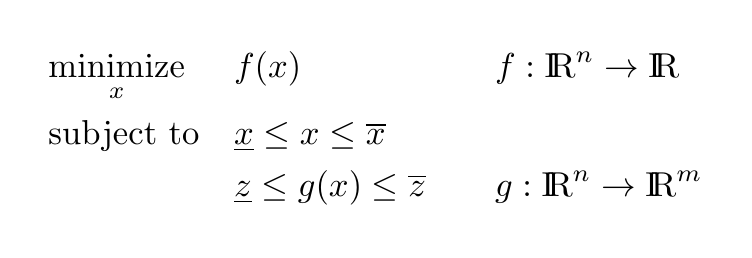
\begin{tikzpicture}[scale=1.25, every node/.style={scale=1.25}]
    \node [inner sep=0.6em] (rec) at (0, 0) {
    \(
        \begin{aligned}
            & \underset{x}{\text{minimize}}
            & & f(x) &&&& f : \Re^n \rightarrow \Re \\
            & \text{subject to}
            & & \underline{x} \le x \le \overline{x} \\
            &&& \underline{z} \le g(x) \le \overline{z} &&&& g : \Re^n \rightarrow \Re^m
        \end{aligned}
        \)
    };
\end{tikzpicture}
\end{document}